% !TEX program = xelatex
% ---------------------------------------------------------------------------
%  The Epitetartic Rhombus  —  a short note
%  Compile with:  xelatex epitetartic_rhombus.tex   (twice)
%  Figures: fig1_arc.pdf, fig2_square.pdf, fig3_halving.pdf  (figs_rhombus.py)
%  Exact checks: verify_rhombus.py
% ---------------------------------------------------------------------------
\documentclass[11pt,a4paper]{article}

\usepackage[margin=2.6cm]{geometry}
\usepackage{amsmath,amsthm,mathtools}
\usepackage{fontspec}
\usepackage{unicode-math}
\setmainfont{Latin Modern Roman}
\setmathfont{Latin Modern Math}
\newfontfamily\greekfont{GFS Porson}[Scale=MatchLowercase]
\usepackage{graphicx}
\usepackage{enumitem}
\usepackage{xcolor}
\usepackage[hidelinks]{hyperref}
\usepackage{caption}
\captionsetup{font=small,labelfont=bf}

\newcommand{\gr}[1]{{\greekfont #1}}

\theoremstyle{plain}
\newtheorem{theorem}{Theorem}
\newtheorem{proposition}[theorem]{Proposition}
\newtheorem{corollary}[theorem]{Corollary}
\theoremstyle{definition}
\newtheorem{definition}[theorem]{Definition}
\theoremstyle{remark}
\newtheorem{remark}[theorem]{Remark}

\hypersetup{
  pdftitle={The Epitetartic Rhombus},
  pdfauthor={Lluis Garcia Torcal},
  pdfkeywords={Fibonacci tiling, Holden's lines, golden spiral, rhombus, 3-4-5 triangle, arctan(4/5)}
}

\begin{document}

\begin{center}
{\LARGE The Epitetartic Rhombus\par}
\vspace{0.3em}
{\large Holden's line, the Fibonacci arc, and a $5:4$ rhombus in every square\par}
\vspace{1.2em}
{\large Lluis Garcia Torcal\par}
\vspace{0.3em}
{\small Independent researcher, Sabadell, Spain \quad·\quad ORCID \href{https://orcid.org/0009-0007-8570-2536}{0009-0007-8570-2536}\\ \href{mailto:lluisgarciamusic@gmail.com}{lluisgarciamusic@gmail.com}\par}
\vspace{0.3em}
{\small Version 3, 20 October 2026 (version 1: 12 October 2026, \href{https://doi.org/10.5281/zenodo.23325443}{doi:10.5281/zenodo.23325443}; version 2: 13 October 2026, \href{https://doi.org/10.5281/zenodo.23327201}{doi:10.5281/zenodo.23327201}) \quad·\quad all versions: \href{https://doi.org/10.5281/zenodo.23325442}{doi:10.5281/zenodo.23325442}\par}
\end{center}

\vspace{0.8em}
\begin{abstract}
\noindent In the Fibonacci tiling, the centres of the squares lie on two perpendicular lines through a point $P$ (Holden, 1975). We show that one of these lines meets the quarter-circle arc of the first unit square exactly at $Q=-P$, the reflection of $P$ through the centre of that square, and that seen from the centre of the arc, $Q$ is a $3$-$4$-$5$ point. More generally, in every square of side $F_k$ Holden's lines cross the arc of the spiral exactly once, at a node of the origins grid exactly $2F_{k+1}$ origins units ($\rho=\sqrt{0.1}$) from $P$, twice the next Fibonacci number, and seen from the centre of that arc the crossing is always the same $3$-$4$-$5$ point, scaled by $F_k$ and turned through $90^\circ$ from one square to the next. This places the angle $\arctan(4/5)$, the slope of the $\pm 4/5$ correction in the author's Pentametric Formula, in every square of the tiling. The rhombus it determines, which grows with the spiral, has diagonals in the ratio $5:4$; we call it the \emph{Epitetartic Rhombus}, after the Greek name of that ratio. We show that the same rhombus can be drawn in any square, with a ruler, from the square's thirds, using both of the angles $\arctan(1/3)$ and $\arctan(1/2)$ of Holden's construction; and that its corner, though it never lands on a halving grid, lands exactly on grids of $15$ and $30$. Version 2 adds the distances from $P$ along the spiral: the crossings all sit $\arctan(4/3)$ into their quarter turn; the joins between consecutive arcs lie exactly $2\sqrt{F_{2j+1}}$ origins units from $P$, the hypotenuse of the two neighbouring crossings; and a square of area $\mathfrak{P}(n)$ whose diagonal points at $P$ misses it by $n-\sqrt{n^2+4(n|5)}$ units, exactly $2\psi^k$ at the Lucas numbers. Version 3 changes no result: it renames the Holden unit and Holden's grid the \emph{origins unit} and the \emph{origins grid}, after the companion note \emph{The Origin of Origins}, where $\sqrt{0.1}$ is the radius of the circle about the centre of the first square through the eight origins, and it states exactly what Holden and Gardiner proved. All statements are elementary and are verified in exact arithmetic.
\end{abstract}

\section{Setting}

We use Gardiner's coordinates \cite{gardiner}: the first Fibonacci square (side $F_1=1$) is centred at the origin, and the centre $C_k$ of the square of side $F_k$ satisfies $C_k - P = i^{\,k-1} L_k\, w$ with $P=(1/10,\,3/10)$ and $w=-(1+3i)/10$, where $L_k$ are the Lucas numbers. Holden \cite{holden} proved that the centres lie alternately on two perpendicular lines, of slopes $3$ and $-1/3$, and gave their distances from the crossing in closed form, $d_i=(f_{i+3}+f_{i-3})/(2\sqrt{10})$; his tables list $d\sqrt{10}$, which for the Fibonacci tiling are the Lucas numbers (he does not name them). Gardiner \cite{gardiner} gave the lines in coordinates centred on the first square:
\[
  y = 3x \qquad\text{and}\qquad x + 3y = 1,
\]
which meet at $P$, with $|C_kP| = L_k/\sqrt{10}$. We call $\rho=\sqrt{0.1}=1/\sqrt{10}$ the \emph{origins unit} \cite{origins} (called the Holden unit in versions 1 and 2): the centre $C_k$ is exactly $L_k$ origins units from $P$. The lines $3x-y=m$ and $x+3y=m$ ($m\in\mathbb{Z}$) form a tilted square grid of side $\rho$ (the \emph{origins grid} \cite{origins}, called Holden's grid in versions 1 and 2; Holden's paper has no grid; cells of area $1/10$); every corner and centre of the tiling, and $P$, are nodes of it. In the author's preprint \cite{gt} the area $L_k^2/5$ of a square through $P$ differs from $F_k^2$ by exactly $\pm 4/5$; drawn as a slope, this correction is the angle $\arctan(4/5)=38.6598^\circ$.

The quarter-circle of the spiral in the first square joins its corners $(-\tfrac12,\tfrac12)$ and $(\tfrac12,-\tfrac12)$ and is centred at the corner $M=(\tfrac12,\tfrac12)$, with radius $1$.

\section{Where Holden's line meets the arc}

\begin{proposition}\label{prop:Q}
The line $y=3x$ meets the circle of the first arc, $(x-\tfrac12)^2+(y-\tfrac12)^2=1$, exactly at the centre $C_3=(\tfrac12,\tfrac32)$ of the third square and at
\[
  Q=\Bigl(-\frac{1}{10},\,-\frac{3}{10}\Bigr) = -P ,
\]
which lies on the arc of the first square. Seen from the arc's centre, $Q-M=(-\tfrac35,-\tfrac45)$ is a $3$-$4$-$5$ vector, and $|PQ| = 2\rho$: $Q$ is two origins units from $P$ along Holden's line, and a node of the grid.
\end{proposition}

\begin{proof}
Substituting $y=3x$ gives $(x-\tfrac12)^2+(3x-\tfrac12)^2-1 = 10x^2-4x-\tfrac12 = \tfrac12(2x-1)(10x+1)$, so $x=\tfrac12$ or $x=-\tfrac1{10}$. The rest is direct computation; $3x-y$ and $x+3y$ are integers at $Q$.
\end{proof}

\begin{remark}
The reason is the double-angle formula: a chord of slope $1/3$ makes the angle $\theta_1=\arctan(1/3)$ with a diameter, so the arc it cuts off subtends $2\theta_1$ at the centre, and $\tan 2\theta_1 = (2/3)/(1-1/9) = 3/4$. Holden's angle produces the $3$-$4$-$5$ triangle, and with it the ratio $4/5$.
\end{remark}

The horizontal line through $Q$ and its mirror image through $M$ cut the vertical diameter at heights $\tfrac12\pm\tfrac45$. Together with the horizontal diameter they give the rhombus
\[
  \mathcal{R} = \bigl(-\tfrac12,\tfrac12\bigr),\ \bigl(\tfrac12,-\tfrac{3}{10}\bigr),\ \bigl(\tfrac32,\tfrac12\bigr),\ \bigl(\tfrac12,\tfrac{13}{10}\bigr),
\]
centred at $M$, with diagonals $2$ and $8/5$ (ratio $5:4$), area $8/5$, and angles $2\arctan(4/5)=77.32^\circ$ and $2\arctan(5/4)=102.68^\circ$. Its first vertex is the corner where the arc starts. It is made of four right triangles with legs $1$ and $4/5$: the $\pm 4/5$ triangle of the correction, standing upright (Figure~\ref{fig:arc}).

\begin{figure}[ht]
\centering
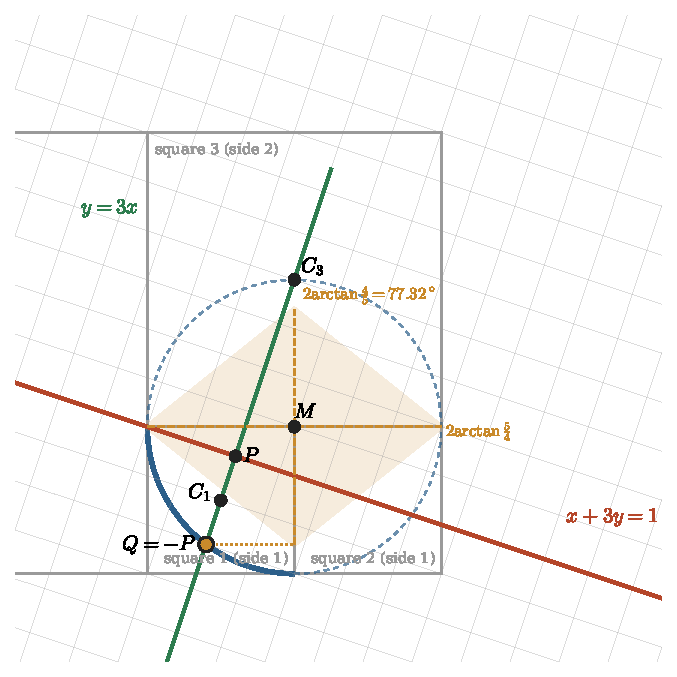
\includegraphics[width=0.62\textwidth]{fig1_arc.pdf}
\caption{Holden's line $y=3x$ (green) meets the arc of the first square at $Q=-P$. The rhombus $\mathcal{R}$ (gold) is centred at the arc's centre $M$. The origins grid of side $\rho=\sqrt{0.1}$ is shown faintly.}
\label{fig:arc}
\end{figure}

\begin{definition}
A rhombus whose diagonals are in the ratio $5:4$ we call an \emph{Epitetartic Rhombus} (\gr{ὁ ἐπιτέταρτος ῥόμβος}), after \gr{ἐπιτέταρτος}, ``a quarter more'', the Greek name of the ratio $5:4$ (the just major third). Its angles are $2\arctan(4/5)$ and $2\arctan(5/4)$, and its side is $\sqrt{41}/10$ of its long diagonal.
\end{definition}

\subsection*{The same crossing in every square}

The arc of the spiral in the square of side $F_k$ is the quarter-circle of radius $F_k$ centred at the corner
\[
  M_k = C_k + F_k\, i^{\,k-1}\,\frac{1+i}{2}
\]
(for $k=1$ this is $M$); this is the standard construction of the spiral, and we checked the formula against the tiling for $k\le 28$.

\begin{theorem}\label{thm:every}
For every $k\ge 1$, the point
\[
  X_k = P + 2F_{k+1}\, i^{\,k-1}\, w
\]
lies on the arc of the square of side $F_k$, and
\[
  X_k - M_k = F_k\, i^{\,k-1}\Bigl(-\frac35-\frac45\,i\Bigr).
\]
So $X_k$ lies on Holden's line through $C_k$ (on the same ray from $P$, $F_k$ origins units beyond the centre, since $2F_{k+1}=L_k+F_k$), it is a node of the origins grid at distance exactly $2F_{k+1}$ origins units from $P$, \emph{twice the next Fibonacci number}, and seen from the centre of its arc it is the $3$-$4$-$5$ point of Proposition~\ref{prop:Q}, scaled by $F_k$ and turned through $90^\circ(k-1)$. $X_1=Q$. The first values (with $n=L_k$, the index at which the Pentametric Formula gives the area $F_k^2$ \cite{gt}):
\begin{center}\small
\begin{tabular}{lcccccccc}
square side $F_k$ & 1 & 1 & 2 & 3 & 5 & 8 & 13 & 21\\
$n = L_k$: centre $C_k$ is $n$ units from $P$ & 1 & 3 & 4 & 7 & 11 & 18 & 29 & 47\\
crossing $X_k$: $2F_{k+1}$ units from $P$ & 2 & 4 & 6 & 10 & 16 & 26 & 42 & 68\\
\end{tabular}
\end{center}
\end{theorem}

\begin{proof}
Since $C_k = P + i^{\,k-1}L_k w$ and $2F_{k+1}-L_k = F_k$,
\[
  X_k - M_k = i^{\,k-1}\Bigl(F_k\,w - F_k\,\tfrac{1+i}{2}\Bigr) = F_k\, i^{\,k-1}\Bigl(-\tfrac{1}{10}-\tfrac12 + \bigl(-\tfrac{3}{10}-\tfrac12\bigr) i\Bigr) = F_k\, i^{\,k-1}\Bigl(-\tfrac35-\tfrac45 i\Bigr),
\]
of modulus $F_k$, so $X_k$ is on the circle. The arc runs from $M_k$'s two neighbouring corners, $M_k - F_k i^{\,k-1}$ and $M_k - F_k i^{\,k}$, so it occupies the directions between $-i^{\,k-1}$ and $-i^{\,k}$ seen from $M_k$; the direction $i^{\,k-1}(-\tfrac35-\tfrac45 i)$ lies strictly between them. Finally $X_k - P$ is an integer multiple of $w$, so $X_k$ is a grid node.
\end{proof}

\begin{remark}
We also checked, for $k\le 28$, that this is the \emph{only} point where Holden's lines meet the arc of the $k$-th square (in the first square the other line also passes through the arc's starting corner $(-\tfrac12,\tfrac12)$, again two steps from $P$). In each square, then, the vertical and horizontal lines through $X_k$ and its mirror image through $M_k$ give an Epitetartic Rhombus centred at $M_k$ with diagonals $2F_k$ and $\tfrac85 F_k$: the rhombus grows with the spiral, by the Fibonacci numbers, and turns with it.
\end{remark}

\begin{figure}[ht]
\centering
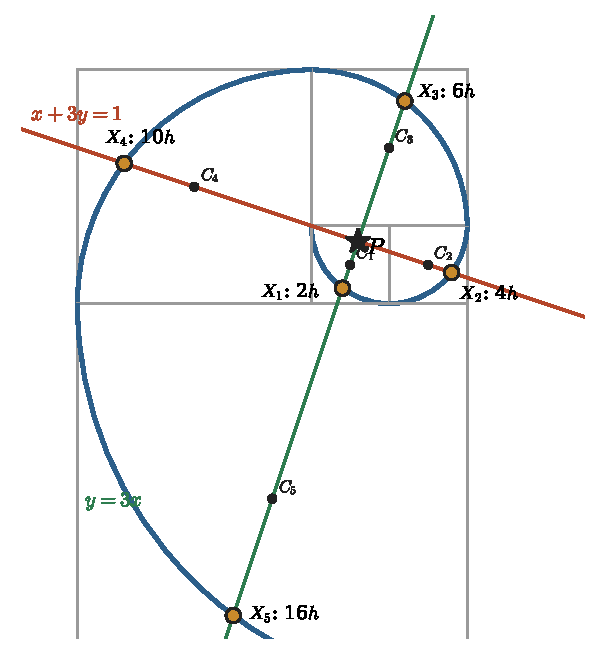
\includegraphics[width=0.66\textwidth]{fig4_crossings.pdf}
\caption{Squares $1$ to $5$ of the tiling with the spiral (blue) and Holden's lines. In each square the spiral crosses Holden's line once, at $X_k$ (gold), exactly $2F_{k+1}$ origins units from $P$: $2, 4, 6, 10, 16$; the centres $C_k$ are $L_k = 1, 3, 4, 7, 11$ units from $P$.}
\label{fig:crossings}
\end{figure}

\section{The Epitetartic Rhombus in any square}

\begin{theorem}\label{thm:square}
In the unit square $[0,1]^2$, the points
\[
  A=\bigl(0,\tfrac13\bigr),\quad B=\bigl(\tfrac{11}{30},\tfrac{9}{10}\bigr),\quad C=\bigl(1,\tfrac23\bigr),\quad D=\bigl(\tfrac{19}{30},\tfrac{1}{10}\bigr)
\]
form an Epitetartic Rhombus centred at the centre of the square. Its long diagonal $AC$ is the line of slope $1/3$ joining the thirds of opposite sides, of length $\sqrt{10}/3$ (it crosses three of the nine small squares). Its short diagonal $BD$ lies on the perpendicular line of slope $-3$ through $(\tfrac13,1)$ and $(\tfrac23,0)$, from height $1/10$ to height $9/10$, so it is $4/5$ of $AC$. Its area is $4/9$ of the square.
\end{theorem}

\begin{proof}
Both diagonals have midpoint $(\tfrac12,\tfrac12)$; $\vec{AC}=(1,\tfrac13)$ and $\vec{BD}=(\tfrac{8}{30},-\tfrac{24}{30})$ are perpendicular, and $|BD|^2/|AC|^2 = (640/900)/(10/9) = 16/25$. The area is $\tfrac12\cdot\tfrac{\sqrt{10}}{3}\cdot\tfrac45\cdot\tfrac{\sqrt{10}}{3} = \tfrac49$.
\end{proof}

\paragraph{Construction with a ruler.} Split the square into $3\times 3$. The line through the middle of the top edge of the top-left small square $(\tfrac16,1)$, the centre of the top-middle small square $(\tfrac12,\tfrac56)$, and the middle of the bottom edge of the top-right small square $(\tfrac56,\tfrac23)$ has slope $-1/2$, the second angle $\theta_2=\arctan(1/2)$ of Holden's construction. It meets the line of slope $-3$ through $(\tfrac13,1)$ where $1-\tfrac12\bigl(x-\tfrac16\bigr) = 1-3\bigl(x-\tfrac13\bigr)$, that is $x-\tfrac16 = 6x-2$, giving $x=\tfrac{11}{30}$, $y=\tfrac{9}{10}$: the corner $B$. The corner $D$ follows by the half-turn about the centre. So both angles of the paper build the rhombus: $\arctan(1/3)$ the long diagonal, $\arctan(1/2)$ the corners (Figure~\ref{fig:square}).

\paragraph{Four in every square.} The two lines of slopes $\pm 1/3$ through the centre, and the two of slopes $\mp 3$, form two perpendicular pairs, and either line of a pair can carry the long diagonal; so every square holds four Epitetartic Rhombi with a common centre.

\begin{corollary}
The rhombus $\mathcal{R}$ of Section~2 is the rhombus of Theorem~\ref{thm:square} drawn in the square of the origins grid of side $6\rho$ centred at $M$ (sides along $(3,-1)$ and $(1,3)$). Its long diagonal joins two nodes of the grid, and its first vertex is the starting corner of the arc.
\end{corollary}

\begin{proof}
Map $[0,1]^2$ onto that square by $(a,b)\mapsto M + 3\bigl((a-\tfrac12)\,u + (b-\tfrac12)\,v\bigr)$ with $u=(\tfrac35,-\tfrac15)$, $v=(\tfrac15,\tfrac35)$ (each of length $2\rho$). The images of $A,B,C,D$ are $(-\tfrac12,\tfrac12)$, $(\tfrac12,\tfrac{13}{10})$, $(\tfrac32,\tfrac12)$, $(\tfrac12,-\tfrac{3}{10})$.
\end{proof}

\begin{figure}[ht]
\centering
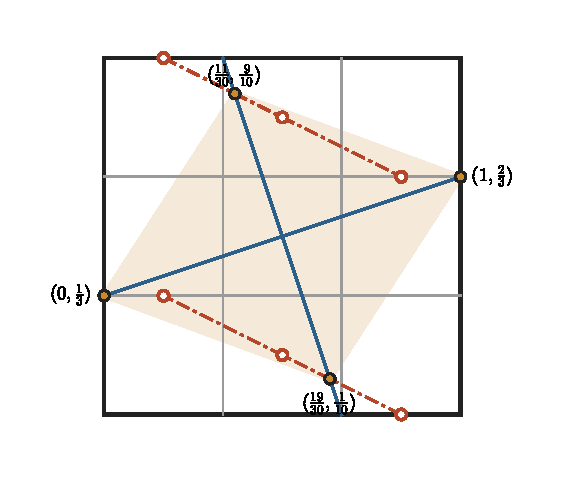
\includegraphics[width=0.48\textwidth]{fig2_square.pdf}
\caption{The Epitetartic Rhombus in a square split $3\times3$. Blue: the two lines of slopes $1/3$ and $-3$. Red: the ruler construction of the corners with lines of slope $-1/2$ through edge middles and a cell centre (open circles).}
\label{fig:square}
\end{figure}

\section{Halving never finds the corner; threes and fives do}

\begin{proposition}
Halving the square repeatedly never makes the corner $B=(\tfrac{11}{30},\tfrac{9}{10})$ a corner or a centre of a cell: in base $2$ both coordinates are purely periodic after two digits, and the quarter that contains $B$ runs top-left, top-right, and then top-left, bottom-right, bottom-right, top-right, repeating with period $4$ (since $2^4\equiv 1 \pmod{15}$). In a grid of $N\times N$ cells, $B$ is a grid corner exactly when $30\mid N$, and the centre of a cell exactly when $N$ is $15$ times an odd number.
\end{proposition}

\begin{proof}
A point is a corner or centre of a cell of a dyadic grid only if its coordinates have a power of $2$ as denominator; $11/30$ and $9/10$ do not. For the $N$-grid, $B$ is a corner iff $11N/30$ and $9N/10$ are integers, i.e.\ $30\mid N$; a centre iff both are half-odd integers, i.e.\ $N=15(2j+1)$.
\end{proof}

\begin{figure}[ht]
\centering
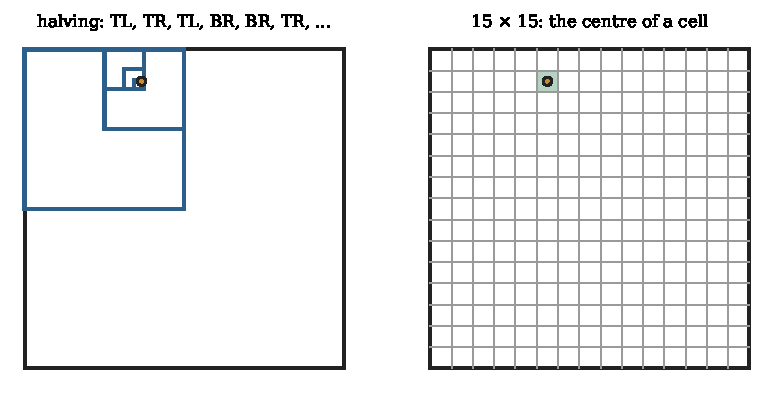
\includegraphics[width=0.7\textwidth]{fig3_halving.pdf}
\caption{Left: the cells of the first six halvings that contain the corner. Right: in the $15\times15$ grid it is the centre of a cell.}
\label{fig:halving}
\end{figure}

\section{Distances from $P$}

Measure every distance from $P$ in origins units $\rho=\sqrt{0.1}$, and parametrise the spiral by $t\ge 0$: for $k-1\le t<k$ the point lies on the arc of the $k$-th square, a fraction $t-(k-1)$ of the way through its quarter turn.

\begin{proposition}[the crossings]\label{prop:angle}
Every crossing $X_k$ of Theorem~\ref{thm:every} lies at the same place of its quarter turn: $\arctan(4/3)=53.13^\circ$ in, the larger acute angle of the $3$-$4$-$5$ triangle.
\end{proposition}

\begin{proof}
Seen from $M_k$ the arc runs from the direction $-i^{\,k-1}$ to $-i^{\,k}$, and $X_k-M_k$ has the direction $i^{\,k-1}(-\tfrac35-\tfrac45 i) = -i^{\,k-1}(\tfrac35+\tfrac45 i)$: the start direction turned by $\arctan(4/3)$.
\end{proof}

\begin{proposition}[the joins]\label{prop:joins}
The arc of the $j$-th square ends, and the arc of the $(j+1)$-th begins, at the corner $A_j = M_j - F_j\, i^{\,j}$, and
\[
  \frac{|PA_j|^2}{\rho^2} = 4F_{2j+1} = (2F_j)^2 + (2F_{j+1})^2 .
\]
So the joins lie $2\sqrt{F_{2j+1}}$ units from $P$ ($2, \sqrt8, \sqrt{20}, \sqrt{52}, \sqrt{136}, \dots$), and each is the hypotenuse of a right triangle whose legs are the distances $2F_j$ and $2F_{j+1}$ of the crossings in the squares on either side.
\end{proposition}

\begin{proof}
$A_j - P = i^{\,j-1}\bigl(L_j w + F_j\tfrac{1+i}{2} - F_j i\bigr) = i^{\,j-1}\bigl(L_j w + F_j\tfrac{1-i}{2}\bigr)$, so
$10\,|A_j-P|^2 = 10\bigl[(\tfrac{F_j}{2}-\tfrac{L_j}{10})^2 + (\tfrac{F_j}{2}+\tfrac{3L_j}{10})^2\bigr] = 5F_j^2 + 2F_jL_j + L_j^2 = (2F_j)^2 + (F_j+L_j)^2$,
and $F_j+L_j = 2F_{j+1}$. Finally $F_j^2+F_{j+1}^2 = F_{2j+1}$.
\end{proof}

\begin{remark}
The spiral starts at $A_0=(-\tfrac12,\tfrac12)$, $2$ units from $P$, comes closest at $\sqrt{10}-\sqrt2 = 1.748$ units (where the line from $M_1$ through $P$ meets the first arc, $29.5\%$ of the way through it), and from there on moves steadily away (checked by sampling for the first $20$ squares), growing by a factor tending to $\varphi$ per quarter turn, since $F_{k+2}/F_{k+1}\to\varphi$ (Figure~\ref{fig:distance}).
\end{remark}

\begin{figure}[ht]
\centering
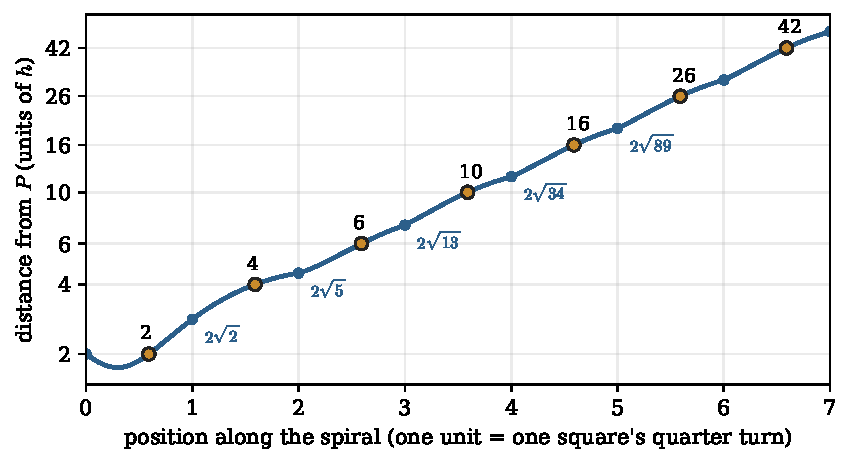
\includegraphics[width=0.78\textwidth]{fig5_distance.pdf}
\caption{Distance from $P$ along the spiral, in origins units (logarithmic scale). Gold: the crossings, $2F_{k+1}$ units, all $\arctan(4/3)$ into their quarter turn. Blue: the joins, $2\sqrt{F_{2j+1}}$ units.}
\label{fig:distance}
\end{figure}

\paragraph{The squares of the Pentametric Formula.} In the author's preprint \cite{gt} the square $S_k$ of area $L_k^2/5$ has its centre at $C_k$, $L_k$ origins units from $P$, and a vertex at $P$. The author's \emph{Pentametric spiral} \cite{site2} extends this to every $n$: a square of area $\mathfrak{P}(n) = (n^2+4\chi(n))/5$, $\chi(n)=(n|5)$, centred $n$ origins units from $P$ with a diagonal pointing at $P$. A square of area $n^2/5$ in that position would have its near corner exactly at $P$ (its half-diagonal is $n/\sqrt{10}$, that is $n$ units).

\begin{proposition}[the near corner]\label{prop:corner}
A square of area $\mathfrak{P}(n)$, centred $n$ origins units from $P$ with a diagonal pointing at $P$, has its near corner
\[
  n-\sqrt{n^2+4\chi(n)}
\]
units from $P$ along that diagonal: past $P$ if $\chi(n)=1$, short of it if $\chi(n)=-1$, exactly at $P$ if $5\mid n$. At the Lucas numbers the miss is exactly
\[
  L_k - \sqrt5\,F_k = 2\psi^k = \pm\frac{2}{\varphi^k}\qquad\Bigl(\psi=\tfrac{1-\sqrt5}{2}\Bigr),
\]
that is $-1.236$, $+0.764$, $-0.472$, $+0.292$, $-0.180, \dots$: it changes side every time and shrinks by the golden ratio. For other $n$ it is close to $\mp 2/n$.
\end{proposition}

\begin{proof}
The half-diagonal of a square of area $A$ is $\sqrt{A/2}$, that is $\sqrt{5A}$ origins units; with $A=\mathfrak{P}(n)$ this is $\sqrt{n^2+4\chi(n)}$. For $n=L_k$, $\chi(L_k)=-(-1)^k$ and $L_k^2-4(-1)^k=5F_k^2$, so the half-diagonal is $\sqrt5\,F_k$, and $L_k-\sqrt5F_k=(\varphi^k+\psi^k)-(\varphi^k-\psi^k)=2\psi^k$.
\end{proof}

\section{Remarks}

\begin{enumerate}[leftmargin=*,itemsep=2pt]
\item All the ingredients are elementary: lines joining the thirds of a square are classical, and the $3$-$4$-$5$ triangle arises from $\arctan(1/3)$ by doubling. What this note records is where they meet in the Fibonacci tiling: the exact point $Q=-P$ on the first arc, the crossing $X_k$ at $2F_{k+1}$ origins units in every square with its constant $3$-$4$-$5$ shape, the rhombus it determines, its placement on the origins grid, and its construction in an arbitrary square.
\item A search among the corners and centres of the tiling alone finds the slope $4/5$ only incidentally \cite{site}; it appears exactly at the intersection of a line with an arc.
\item The figures in the author's GeoGebra files use the frame $(x,y)\mapsto(-\tfrac12+y,\,-\tfrac12-x)$ of Gardiner's coordinates, in which $P=(-\tfrac15,-\tfrac35)$, $Q=(-\tfrac45,-\tfrac25)$ and the arc is centred at $(0,-1)$.
\item \sloppy Interactive figures:\\ \url{https://lluisgarcia.github.io/The-Pentametric-Cycle/rhombus.html} and\\ \url{https://lluisgarcia.github.io/The-Pentametric-Cycle/distance.html}.\\ GeoGebra files, images and the exact checks (verify\_rhombus.py, crossings.py, distances.py; figures figs\_rhombus.py, fig4.py, fig5.py):\\ \url{https://github.com/lluisgarcia/The-Pentametric-Cycle}.
\end{enumerate}

\paragraph{Acknowledgements and use of AI.} The constructions, the question of the distance from $P$ to the spiral, the observation that Holden's lines cross the arc of every square once, at twice the next Fibonacci number of origins units from $P$, and the name are the author's, found in GeoGebra. Claude (Anthropic, Opus 5.5) was used to verify the statements in exact arithmetic, to prepare the figures and to help draft the text; the author checked and approved every statement.

\paragraph{Licence.} This note is released under CC BY 4.0; the accompanying Python scripts under the MIT licence.

\begin{thebibliography}{9}
\bibitem{holden} H.~L. Holden, Fibonacci tiles, \emph{The Fibonacci Quarterly} \textbf{13} (1975) 45--49.
\bibitem{gardiner} T. Gardiner, 68.15 The Fibonacci spiral, \emph{The Mathematical Gazette} \textbf{68} (1984) 120.
\bibitem{gt} L. Garcia Torcal, \emph{The Pentametric Cycle: A Nested Palindrome Encoding the Pythagorean Consonances}, preprint, Zenodo (2026), \href{https://doi.org/10.5281/zenodo.23183108}{doi:10.5281/zenodo.23183108}.
\bibitem{site2} L. Garcia Torcal, \emph{The Pentametric spiral}, interactive page, \url{https://lluisgarcia.github.io/The-Pentametric-Cycle/pentaspiral.html} (2026).
\bibitem{origins} L. Garcia Torcal, \emph{The Origin of Origins: How a circle of area $\pi/10$ about the centre of the unit square gives eight origins, one for each of eight Fibonacci spirals}, note, Zenodo (2026), \href{https://doi.org/10.5281/zenodo.23486276}{doi:10.5281/zenodo.23486276}.
\bibitem{site} L. Garcia Torcal, \emph{The angle of 0.8}, interactive page, \url{https://lluisgarcia.github.io/The-Pentametric-Cycle/angle.html} (2026).
\end{thebibliography}

\end{document}
